\begin{tikzpicture} 
\only<1|handout:1>{
\begin{axis}[
name=ideal_lpf_td,
anchor=origin,
axis lines*=middle,
enlargelimits = true,
ymin=-0.1,
ymax=1.2*0.5,
xmin=-10,
xmax=10,
axis line style={->,>=stealth},
xlabel={$n$},
ylabel={$h_{lpf}[n]$},
yticklabel style = {yshift=0.2cm},
xticklabel style = {yshift=-0.1cm},
every axis x label/.style={
	at={(ticklabel* cs:1)},
	anchor=north,
},
every axis y label/.style={
	at={(ticklabel* cs:1)},
	anchor=south,
},
ytick=0.5,
yticklabels={$\frac{\omega_c}{\pi}$},
xtick=\empty,
every outer y axis line/.append style={white!15!black},
every y tick label/.append style={font=\color{white!15!black}},
legend style={draw=white!15!black,fill=white,legend cell align=left}]

\addplot[ycomb, mark=*, fill=white, mark options={scale=1.5, fill=white}, line width=1.5pt, domain=-10:10, samples=21] {sin(deg(pi/2*x))/(pi*x) + 1/2*(x == 0)};
\addplot[smooth, black!20, line width=1pt, domain=-10:10, samples=21] {sin(deg(pi/2*x))/(pi*x) + 1/2*(x == 0)};
\end{axis}

\begin{axis}[
name=ideal_lpf_fd,
at=(ideal_lpf_td.right of south east), anchor=left of south west, xshift=1.2cm,
axis lines*=middle,
enlargelimits = true,
xmax=4,
xmin=-4,
ymin=-0.2,
ymax=1.2,
axis line style={->,>=stealth},
xlabel={$\omega$},
ylabel={$H_{lpf}(e^{j\omega})$},
yticklabel style = {yshift=0.2cm},
xticklabel style = {yshift=-0.3cm},
every axis x label/.style={
    at={(ticklabel* cs:1)},
    anchor=north,
},
every axis y label/.style={
    at={(ticklabel* cs:1)},
    anchor=south,
},
xtick=\empty,
ytick={1},
xtick={-3.14, -1.5708, 1.5708, 3.14},
xticklabels={$-\pi$, $-\omega_c$, $\omega_c$, $\pi$},
every outer y axis line/.append style={white!15!black},
every y tick label/.append style={font=\color{white!15!black}},
legend style={draw=white!15!black,fill=white,legend cell align=left}]

	\addplot[black, domain=-pi/2:pi/2, samples=2,line width=2pt] {1};
	\addplot[black, line width=2pt] coordinates {(-pi/2, 0) (-pi/2, 1.01)};
	\addplot[black, domain=-pi:-pi/2, samples=2,line width=2pt] {0};
	\addplot[black, domain=pi/2:pi, samples=2,line width=2pt] {0};
	\addplot[black, line width=2pt] coordinates {(pi/2, 0) (pi/2, 1.01)};
\end{axis}
}

%%%%%%%%%%%%%%%%%% 
\only<2|handout:2>{
	\begin{axis}[
	name=truncated_lpf_td,
	anchor=origin,
	axis lines*=middle,
	enlargelimits = true,
	ymin=-0.1,
	ymax=1.2*0.5,
	xmin=-7,
	xmax=7,
	axis line style={->,>=stealth},
	xlabel={$n$},
	ylabel={$h_{lpf}[n]$},
	yticklabel style = {yshift=0.2cm},
	xticklabel style = {yshift=0.6cm},
	every axis x label/.style={
		at={(ticklabel* cs:1)},
		anchor=north,
	},
	every axis y label/.style={
		at={(ticklabel* cs:1)},
		anchor=south,
	},
	ytick=0.5,
	yticklabels={$\frac{\omega_c}{\pi}$},
	xtick={-7, 7},
	xticklabels={\tikz[baseline]{\node[fill=blue!20,anchor=base,scale=0.7] {$-M$};}, \tikz[baseline]{\node[fill=blue!20,anchor=base,scale=0.7] {$M$};}},
	every outer y axis line/.append style={white!15!black},
	every y tick label/.append style={font=\color{white!15!black}},
	legend style={draw=white!15!black,fill=white,legend cell align=left}]
	
	\addplot[ycomb, mark=*, fill=white, mark options={scale=1.5, fill=white}, line width=1.5pt, domain=-7:7, samples=15] {sin(deg(pi/2*x))/(pi*x) + 1/2*(x == 0)};
	\addplot[smooth, black!20, line width=1pt, domain=-7:7, samples=15] {sin(deg(pi/2*x))/(pi*x) + 1/2*(x == 0)};
	\end{axis}
	
	\begin{axis}[
	name=truncated_lpf_fd,
	at=(truncated_lpf_td.right of south east), anchor=left of south west, xshift=1.2cm,
	axis lines*=middle,
	enlargelimits = true,
	xmax=4,
	xmin=-4,
	ymin=-0.2,
	ymax=1.2,
	axis line style={->,>=stealth},
	xlabel={$\omega$},
	ylabel={$H_{lpf}(e^{j\omega})$},
	yticklabel style = {yshift=0.2cm},
	xticklabel style = {yshift=-0.3cm},
	every axis x label/.style={
		at={(ticklabel* cs:1)},
		anchor=north,
	},
	every axis y label/.style={
		at={(ticklabel* cs:1)},
		anchor=south,
	},
	xtick=\empty,
	ytick={1},
	xtick={-3.14, -1.5708, 1.5708, 3.14},
	xticklabels={$-\pi$, $-\omega_c$, $\omega_c$, $\pi$},
	every outer y axis line/.append style={white!15!black},
	every y tick label/.append style={font=\color{white!15!black}},
	legend style={draw=white!15!black,fill=white,legend cell align=left}]
	
	\addplot[black!20, domain=-pi/2:pi/2, samples=2,line width=2pt] {1};
	\addplot[black!20, line width=2pt] coordinates {(-pi/2, 0) (-pi/2, 1.01)};
	\addplot[black!20, domain=-pi:-pi/2, samples=2,line width=2pt] {0};
	\addplot[black!20, domain=pi/2:pi, samples=2,line width=2pt] {0};
	\addplot[black!20, line width=2pt] coordinates {(pi/2, 0) (pi/2, 1.01)};
	
	\addplot [color=black, solid, line width=1.5pt, forget plot]
	table[row sep=crcr]{
		-3.1416 0.039209 \\
		-3.0781 0.034184 \\
		-3.0147 0.020324 \\
		-2.9512 0.00099044 \\
		-2.8877 -0.019066 \\
		-2.8243 -0.0348 \\
		-2.7608 -0.042056 \\
		-2.6973 -0.038583 \\
		-2.6339 -0.024655 \\
		-2.5704 -0.0031491 \\
		-2.5069 0.020968 \\
		-2.4435 0.041656 \\
		-2.38 0.053128 \\
		-2.3165 0.051242 \\
		-2.2531 0.034652 \\
		-2.1896 0.0054863 \\
		-2.1261 -0.030621 \\
		-2.0627 -0.065184 \\
		-1.9992 -0.088127 \\
		-1.9357 -0.089437 \\
		-1.8723 -0.060929 \\
		-1.8088 0.0022081 \\
		-1.7453 0.10035 \\
		-1.6819 0.22911 \\
		-1.6184 0.37975 \\
		-1.5549 0.54037 \\
		-1.4915 0.69762 \\
		-1.428 0.83864 \\
		-1.3645 0.95293 \\
		-1.3011 1.0338 \\
		-1.2376 1.0793 \\
		-1.1741 1.0921 \\
		-1.1107 1.0788 \\
		-1.0472 1.0487 \\
		-0.98373 1.0122 \\
		-0.92026 0.97863 \\
		-0.8568 0.95526 \\
		-0.79333 0.94598 \\
		-0.72986 0.95114 \\
		-0.6664 0.96788 \\
		-0.60293 0.99105 \\
		-0.53947 1.0146 \\
		-0.476 1.0328 \\
		-0.41253 1.0417 \\
		-0.34907 1.0397 \\
		-0.2856 1.0278 \\
		-0.22213 1.0093 \\
		-0.15867 0.98893 \\
		-0.0952 0.97181 \\
		-0.031733 0.96207 \\
		0.031733 0.96207 \\
		0.0952 0.97181 \\
		0.15867 0.98893 \\
		0.22213 1.0093 \\
		0.2856 1.0278 \\
		0.34907 1.0397 \\
		0.41253 1.0417 \\
		0.476 1.0328 \\
		0.53947 1.0146 \\
		0.60293 0.99105 \\
		0.6664 0.96788 \\
		0.72986 0.95114 \\
		0.79333 0.94598 \\
		0.8568 0.95526 \\
		0.92026 0.97863 \\
		0.98373 1.0122 \\
		1.0472 1.0487 \\
		1.1107 1.0788 \\
		1.1741 1.0921 \\
		1.2376 1.0793 \\
		1.3011 1.0338 \\
		1.3645 0.95293 \\
		1.428 0.83864 \\
		1.4915 0.69762 \\
		1.5549 0.54037 \\
		1.6184 0.37975 \\
		1.6819 0.22911 \\
		1.7453 0.10035 \\
		1.8088 0.0022081 \\
		1.8723 -0.060929 \\
		1.9357 -0.089437 \\
		1.9992 -0.088127 \\
		2.0627 -0.065184 \\
		2.1261 -0.030621 \\
		2.1896 0.0054863 \\
		2.2531 0.034652 \\
		2.3165 0.051242 \\
		2.38 0.053128 \\
		2.4435 0.041656 \\
		2.5069 0.020968 \\
		2.5704 -0.0031491 \\
		2.6339 -0.024655 \\
		2.6973 -0.038583 \\
		2.7608 -0.042056 \\
		2.8243 -0.0348 \\
		2.8877 -0.019066 \\
		2.9512 0.00099044 \\
		3.0147 0.020324 \\
		3.0781 0.034184 \\
		3.1416 0.039209 \\
	};
	
	\node at (axis cs: 3.14, 1.1) {\Large \tikz[baseline]{
			\node[fill=blue!20,anchor=base] (t1) {$M = 7$}}};
	
	\end{axis}
}

%%%%%%%%%%%%%%%%%% 
\only<3|handout:3>{
	\begin{axis}[
	name=truncated_lpf_td,
	anchor=origin,
	axis lines*=middle,
	enlargelimits = true,
	ymin=-0.1,
	ymax=1.2*0.5,
	xmin=-19,
	xmax=19,
	axis line style={->,>=stealth},
	xlabel={$n$},
	ylabel={$h_{lpf}[n]$},
	yticklabel style = {yshift=0.2cm},
	xticklabel style = {yshift=0.6cm},
	every axis x label/.style={
		at={(ticklabel* cs:1)},
		anchor=north,
	},
	every axis y label/.style={
		at={(ticklabel* cs:1)},
		anchor=south,
	},
	ytick=0.5,
	yticklabels={$\frac{\omega_c}{\pi}$},
	xtick={-19, 19},
	xticklabels={\tikz[baseline]{\node[fill=blue!20,anchor=base,scale=0.7] {$-M$};}, \tikz[baseline]{\node[fill=blue!20,anchor=base,scale=0.7] {$M$};}},
	every outer y axis line/.append style={white!15!black},
	every y tick label/.append style={font=\color{white!15!black}},
	legend style={draw=white!15!black,fill=white,legend cell align=left}]
	
	\addplot[ycomb, mark=*, fill=white, mark options={scale=1.5, fill=white}, line width=1.5pt,  domain=-19:19, samples=39] {sin(deg(pi/2*x))/(pi*x) + 1/2*(x == 0)};
	\addplot[smooth, black!20, line width=1pt, domain=-19:19, samples=39] {sin(deg(pi/2*x))/(pi*x) + 1/2*(x == 0)};
	\end{axis}
	
	\begin{axis}[
	name=truncated_lpf_fd,
	at=(truncated_lpf_td.right of south east), anchor=left of south west, xshift=1.2cm,
	axis lines*=middle,
	enlargelimits = true,
	xmax=4,
	xmin=-4,
	ymin=-0.2,
	ymax=1.2,
	axis line style={->,>=stealth},
	xlabel={$\omega$},
	ylabel={$H_{lpf}(e^{j\omega})$},
	yticklabel style = {yshift=0.2cm},
	xticklabel style = {yshift=-0.3cm},
	every axis x label/.style={
		at={(ticklabel* cs:1)},
		anchor=north,
	},
	every axis y label/.style={
		at={(ticklabel* cs:1)},
		anchor=south,
	},
	xtick=\empty,
	ytick={1},
	xtick={-3.14, -1.5708, 1.5708, 3.14},
	xticklabels={$-\pi$, $-\omega_c$, $\omega_c$, $\pi$},
	every outer y axis line/.append style={white!15!black},
	every y tick label/.append style={font=\color{white!15!black}},
	legend style={draw=white!15!black,fill=white,legend cell align=left}]
	
	\addplot[black!20, domain=-pi/2:pi/2, samples=2,line width=2pt] {1};
	\addplot[black!20, line width=2pt] coordinates {(-pi/2, 0) (-pi/2, 1.01)};
	\addplot[black!20, domain=-pi:-pi/2, samples=2,line width=2pt] {0};
	\addplot[black!20, domain=pi/2:pi, samples=2,line width=2pt] {0};
	\addplot[black!20, line width=2pt] coordinates {(pi/2, 0) (pi/2, 1.01)};
	
	\addplot [color=black, solid, line width=1.5pt, forget plot]
table[row sep=crcr]{
	-3.1416 0.015876 \\
	-3.11 0.012806 \\
	-3.0784 0.0047726 \\
	-3.0469 -0.0051424 \\
	-3.0153 -0.013122 \\
	-2.9837 -0.01607 \\
	-2.9521 -0.012801 \\
	-2.9206 -0.0045107 \\
	-2.889 0.0056547 \\
	-2.8574 0.013781 \\
	-2.8259 0.016676 \\
	-2.7943 0.013113 \\
	-2.7627 0.0043342 \\
	-2.7311 -0.006365 \\
	-2.6996 -0.014863 \\
	-2.668 -0.017776 \\
	-2.6364 -0.013789 \\
	-2.6048 -0.0042266 \\
	-2.5733 0.0073679 \\
	-2.5417 0.016523 \\
	-2.5101 0.019535 \\
	-2.4785 0.014937 \\
	-2.447 0.0041704 \\
	-2.4154 -0.0088347 \\
	-2.3838 -0.019057 \\
	-2.3522 -0.022276 \\
	-2.3207 -0.016768 \\
	-2.2891 -0.004133 \\
	-2.2575 0.011106 \\
	-2.226 0.023056 \\
	-2.1944 0.026652 \\
	-2.1628 0.019706 \\
	-2.1312 0.0040161 \\
	-2.0997 -0.01496 \\
	-2.0681 -0.029875 \\
	-2.0365 -0.034159 \\
	-2.0049 -0.024686 \\
	-1.9734 -0.0034348 \\
	-1.9418 0.022586 \\
	-1.9102 0.043309 \\
	-1.8786 0.049014 \\
	-1.8471 0.034142 \\
	-1.8155 0.00025733 \\
	-1.7839 -0.042935 \\
	-1.7523 -0.079062 \\
	-1.7208 -0.08885 \\
	-1.6892 -0.055218 \\
	-1.6576 0.031713 \\
	-1.6261 0.1712 \\
	-1.5945 0.35111 \\
	-1.5629 0.55018 \\
	-1.5313 0.74274 \\
	-1.4998 0.90461 \\
	-1.4682 1.0186 \\
	-1.4366 1.0783 \\
	-1.405 1.0884 \\
	-1.3735 1.0631 \\
	-1.3419 1.0211 \\
	-1.3103 0.98084 \\
	-1.2787 0.95576 \\
	-1.2472 0.95147 \\
	-1.2156 0.96573 \\
	-1.184 0.99043 \\
	-1.1524 1.0152 \\
	-1.1209 1.0311 \\
	-1.0893 1.0336 \\
	-1.0577 1.0234 \\
	-1.0261 1.0055 \\
	-0.99457 0.98732 \\
	-0.963 0.97552 \\
	-0.93143 0.97388 \\
	-0.89985 0.98214 \\
	-0.86828 0.99648 \\
	-0.83671 1.0111 \\
	-0.80513 1.0206 \\
	-0.77356 1.0217 \\
	-0.74198 1.0146 \\
	-0.71041 1.0024 \\
	-0.67884 0.98987 \\
	-0.64726 0.98183 \\
	-0.61569 0.98105 \\
	-0.58412 0.98748 \\
	-0.55254 0.99841 \\
	-0.52097 1.0095 \\
	-0.48939 1.0166 \\
	-0.45782 1.0172 \\
	-0.42625 1.0111 \\
	-0.39467 1.001 \\
	-0.3631 0.99079 \\
	-0.33152 0.98432 \\
	-0.29995 0.98398 \\
	-0.26838 0.98979 \\
	-0.2368 0.99942 \\
	-0.20523 1.0091 \\
	-0.17366 1.0152 \\
	-0.14208 1.0154 \\
	-0.11051 1.0096 \\
	-0.078934 1.0002 \\
	-0.047361 0.99075 \\
	-0.015787 0.98491 \\
	0.015787 0.98491 \\
	0.047361 0.99075 \\
	0.078934 1.0002 \\
	0.11051 1.0096 \\
	0.14208 1.0154 \\
	0.17366 1.0152 \\
	0.20523 1.0091 \\
	0.2368 0.99942 \\
	0.26838 0.98979 \\
	0.29995 0.98398 \\
	0.33152 0.98432 \\
	0.3631 0.99079 \\
	0.39467 1.001 \\
	0.42625 1.0111 \\
	0.45782 1.0172 \\
	0.48939 1.0166 \\
	0.52097 1.0095 \\
	0.55254 0.99841 \\
	0.58412 0.98748 \\
	0.61569 0.98105 \\
	0.64726 0.98183 \\
	0.67884 0.98987 \\
	0.71041 1.0024 \\
	0.74198 1.0146 \\
	0.77356 1.0217 \\
	0.80513 1.0206 \\
	0.83671 1.0111 \\
	0.86828 0.99648 \\
	0.89985 0.98214 \\
	0.93143 0.97388 \\
	0.963 0.97552 \\
	0.99457 0.98732 \\
	1.0261 1.0055 \\
	1.0577 1.0234 \\
	1.0893 1.0336 \\
	1.1209 1.0311 \\
	1.1524 1.0152 \\
	1.184 0.99043 \\
	1.2156 0.96573 \\
	1.2472 0.95147 \\
	1.2787 0.95576 \\
	1.3103 0.98084 \\
	1.3419 1.0211 \\
	1.3735 1.0631 \\
	1.405 1.0884 \\
	1.4366 1.0783 \\
	1.4682 1.0186 \\
	1.4998 0.90461 \\
	1.5313 0.74274 \\
	1.5629 0.55018 \\
	1.5945 0.35111 \\
	1.6261 0.1712 \\
	1.6576 0.031713 \\
	1.6892 -0.055218 \\
	1.7208 -0.08885 \\
	1.7523 -0.079062 \\
	1.7839 -0.042935 \\
	1.8155 0.00025733 \\
	1.8471 0.034142 \\
	1.8786 0.049014 \\
	1.9102 0.043309 \\
	1.9418 0.022586 \\
	1.9734 -0.0034348 \\
	2.0049 -0.024686 \\
	2.0365 -0.034159 \\
	2.0681 -0.029875 \\
	2.0997 -0.01496 \\
	2.1312 0.0040161 \\
	2.1628 0.019706 \\
	2.1944 0.026652 \\
	2.226 0.023056 \\
	2.2575 0.011106 \\
	2.2891 -0.004133 \\
	2.3207 -0.016768 \\
	2.3522 -0.022276 \\
	2.3838 -0.019057 \\
	2.4154 -0.0088347 \\
	2.447 0.0041704 \\
	2.4785 0.014937 \\
	2.5101 0.019535 \\
	2.5417 0.016523 \\
	2.5733 0.0073679 \\
	2.6048 -0.0042266 \\
	2.6364 -0.013789 \\
	2.668 -0.017776 \\
	2.6996 -0.014863 \\
	2.7311 -0.006365 \\
	2.7627 0.0043342 \\
	2.7943 0.013113 \\
	2.8259 0.016676 \\
	2.8574 0.013781 \\
	2.889 0.0056547 \\
	2.9206 -0.0045107 \\
	2.9521 -0.012801 \\
	2.9837 -0.01607 \\
	3.0153 -0.013122 \\
	3.0469 -0.0051424 \\
	3.0784 0.0047726 \\
	3.11 0.012806 \\
	3.1416 0.015876 \\
};
	
	\node at (axis cs: 3.14, 1.1) {\Large \tikz[baseline]{
			\node[fill=blue!20,anchor=base] (t1) {$M = 19$}}};
	
	\end{axis}
}

\end{tikzpicture}